\documentclass[14pt]{extarticle}
% math symbols
\usepackage{sfg}


\usepackage{amssymb,amsmath}
\synctex=1
% for different compilers
\usepackage{ifpdf}
% geometry of page
\usepackage[margin=2cm]{geometry}

% if pdflatex, then
\ifpdf
\usepackage[russian]{babel}
\usepackage[utf8]{inputenc}
\usepackage[unicode]{hyperref}
\usepackage[pdftex]{graphicx}
\usepackage{cmlgc}
% if xelatex, then
\else
% math fonts
\usepackage{fouriernc}
% xelatex specific packages
\usepackage[xetex]{hyperref}
\usepackage{xltxtra}	% \XeLaTeX macro
\usepackage{xunicode}	% some extra unicode support
\defaultfontfeatures{Mapping=tex-text}
\usepackage{polyglossia}	% instead of babel in xelatex
\usepackage{indentfirst}	% 
\setdefaultlanguage{russian}
% fonts
\newfontfamily\cyrillicfont{SchoolBookC}
\newfontfamily\cyrillicfontsf{TextBookC}
\setmonofont{Consolas}
\fi

% several pictures in one figure
\usepackage{subfig}
% calc in TeX expressions
\usepackage{calc}
% nice pictures and plots
\usepackage{pgfplots,tikz,circuitikz}
% different libraries for pictures
\usetikzlibrary{%
  arrows,%
  calc,%
  patterns,%
  decorations.pathreplacing,%
  decorations.pathmorphing,%
  decorations.markings,%
  intersections,%
  decorations.text%
}

\usepackage{tkz-euclide}

\usepackage{enumitem}
\renewcommand{\theenumi}{(\asbuk{enumi})}
\renewcommand{\labelenumi}{\asbuk{enumi})}
\AddEnumerateCounter{\Asbuk}{\@Asbuk}{\CYRM}
\AddEnumerateCounter{\asbuk}{\@asbuk}{\cyrm}

\begin{document}

\section*{Задача}

\subsection*{Условие}
Пусть отрезок $PO$ -- перпендикуляр к плоскости $\alpha$, $O\in\alpha$. Пусть $PA$, $PB$, $PC$ -- разные наклонные к этой плоскости, образующие между собой равные углы. Как вычислить угол между этими наклонными, если известны длина перпендикуляра к плоскости и длины наклонных? Для этой же ситуации составьте задачи, обратные данной.
\subsection*{Решение}
Заметим, что $\triangle APC = \triangle CPB = \triangle APB$. Как следствие $\triangle ABC$ равносторонний. Пусть $OP=h$, $PC=PB=PA=a$. Из теоремы пифагора следует, что $b=OA=OC=OB=\sqrt{a^2-h^2}$. Также $c=AC=\sqrt{3}*b$. Так как $\triangle APC$ равнобедренный, $2sin(\alpha/2)=c/a \Rightarrow \alpha=2asin(\frac{c}{2a})$.
\newpage
\begin{figure}[h]
	\centering
	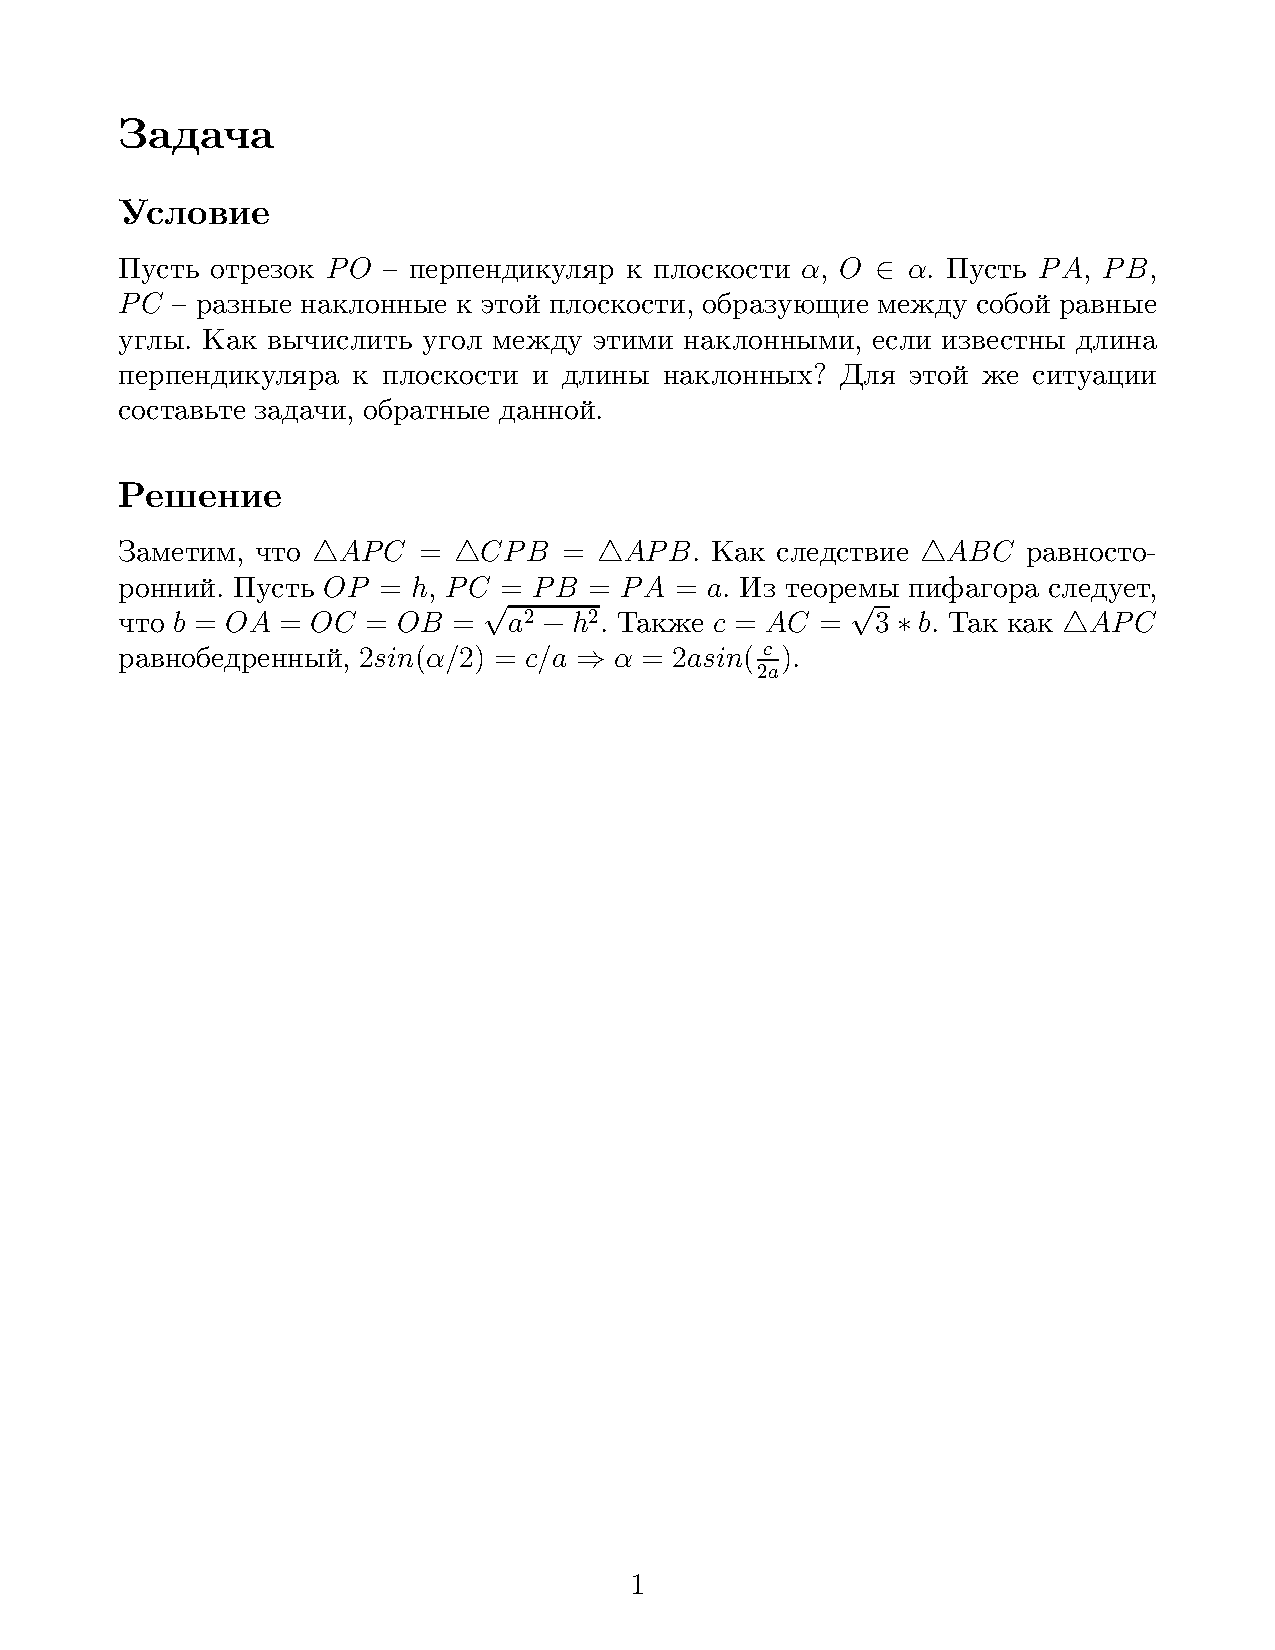
\includegraphics[width=1\textwidth]{{/home/galqiwi/geoma/7.12}.png}
\end{figure}


\end{document}